
\subsection*{task 2.3 \\[1ex] superpixels (part 1)}

In the previous task, we have already seen examples of images composed of \emph{superpixels}. These are images of size $M \times N$ whose content consists of uniformly colored tiles of size $m \times n$ where $m \ll M$ and $n \ll N$.

In the previous task, the superpixels resulted from (na\"ively) upsampling a small image into a larger one. However, superpixels also arise in an image effect called \emph{pixelize} (which is often used to render faces unrecognizable). In this effect, each pixel in each $m \times n$ tile of a given image is set to the average intensity value within the tile.

\begin{figure}[h!]
\subfloat[given image]{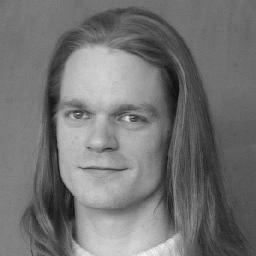
\includegraphics[width=0.32\textwidth]{portrait.png}} \hfill
\subfloat[$8 \times 8$ pixelize]{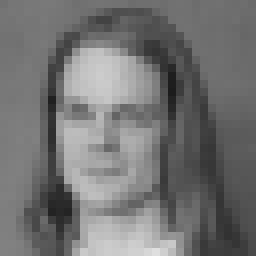
\includegraphics[width=0.32\textwidth]{t2-3-8x8.png}} \hfill
\subfloat[$16 \times 16$ pixelize]{
\includegraphics[width=0.32\textwidth]{t2-3-16x16.png}} 
\end{figure}

\vfill
As always, there are many ways for how to implement this effect. Here is an intuitive C-style implementation that involves four nested \keyword{for} loops
\begin{python}[emph={meanSuperPixelV1,meanSuperPixelV2,meanSuperPixelV3,meanSuperPixelV4}]
def meanSuperPixelV1(arrF, m, n):
    M, N = arrF.shape
    
    arrG = np.zeros((M, N))

    for i in range(0, M, m):
        for j in range(0, N, n):
            intensity_sum = 0
            for k in range(m):
                for l in range(n):
                    intensity_sum += arrF[i+k,j+l]
            intensity_avg = intensity_sum / (m*n)
            arrG[i:i+m,j:j+n] = intensity_avg

    return arrG
\end{python}

\newpage
We don have to be quite so na\"ive but can replace the two innermost \keyword{for} loops using the \emph{numpy} function \keyword{np.mean()}
\begin{python}[emph={meanSuperPixelV1,meanSuperPixelV2,meanSuperPixelV3,meanSuperPixelV4}]
def meanSuperPixelV2(arrF, m, n):
    M, N = arrF.shape
    
    arrG = np.zeros((M, N))

    for i in range(0, M, m):
        for j in range(0, N, n):
            arrG[i:i+m,j:j+n] = np.mean(arrF[i:i+m,j:j+n])

    return arrG
\end{python}

As almost always, \emph{numpy} allows us to get rid of \keyword{for} loops alltogether. Here is a solution inspired by the kind of (unfortunately often stupid) answers you will get when asking the \href{https://stackoverflow.com/questions/14229029/block-mean-of-numpy-2d-array}{\textbf{stackoverflow}} community (we will not even bother discussing this messy mumble \ldots)

\begin{python}[emph={meanSuperPixelV1,meanSuperPixelV2,meanSuperPixelV3,meanSuperPixelV4}]
def meanSuperPixelV3(arrF, m, n):
    M, N = arrF.shape

    arrG = np.reshape(arrF, (M*N//n, n))
    arrG = np.mean(arrG, axis=1)
    arrG = np.reshape(arrG, (M,N//n))

    arrH = np.reshape(arrG, (m, (M//m)*(N//n)), 'F')
    arrH = np.mean(arrH, axis=0)
    arrH = np.reshape(arrH, (M//m, N//n), 'F')

    return np.kron(arrH, np.ones((m,n)))
\end{python}    

Finally, here is how \emph{numpy} black belts implement the pixelize effect (we will discuss this coding pattern later in the course)
\begin{python}[emph={meanSuperPixelV1,meanSuperPixelV2,meanSuperPixelV3,meanSuperPixelV4}]   
def meanSuperPixelV4(arrF, m, n):
    M, N = arrF.shape

    arrA = np.add.reduceat(arrF, np.arange(0,N,n), axis=1) / n
    arrB = np.add.reduceat(arrA, np.arange(0,M,m), axis=0) / m
    arrC = np.repeat(arrB, n, axis=1)
    arrD = np.repeat(arrC, m, axis=0)
    
    return arrD
\end{python}

\textbf{Here is your task:} letting $m=n=8$,  perform runtime measurements for the above four methods on \texttt{portrait.png} and enter your results here
\color{blue} \\[1ex]
%%%%%
%%%%%
%%%%% enter your result here
%%%%%
%%%%%
enter your result here \ldots
%%%%%
%%%%%
%%%%%
%%%%%
%%%%%
\color{black}




